\chapter{Implementazione di un MLP} % Main chapter title
\label{Capitolo2} % Change X to a consecutive number; for referencing this chapter elsewhere, use \ref{ChapterX}
%variables to define path to images
\def \path {Figures/C1}
\def \teoria {Figures/teoria}
%Parlare brevemente del caso di studio
Per il caso di studio introdotto nel Capitolo \ref{Capitolo1} si è implementato da zero un percettrone multistrato a 3 strati come quello illustrato in sezione \ref{sec:mlp}. Vediamo qui di seguito le varie parti da implementare passo passo per costruire un MLP, addestrarlo e verificare che l'addestramento sia stato eseguito in maniera corretta. Il progetto è realizzato in Lua, per utilizzare il framework per il \emph{Machine Learning} \textbf{Torch}(si veda l'appendice\ref{AppendixB}) e mantenere le consistenza con i capitoli successivi, nei quali si userà ancora Torch per addestrare reti neurali molto più complesse.

%--------------------------------------------------------------------
%	SECTION 1
%--------------------------------------------------------------------
\section{Dataset e Architettura}
Nei vari anni, Loris ha cambiato le due variabili in gioco annotando di volta in volta i risultati. Siccome i coperti erano troppo pochi e le file d'attesa erano troppo lunghe, il ristorante perdeva alcuni clienti. Quindi Loris ha portato i coperti a 25 e diminuendo le ore settimanali a 38, ed i profitti sono aumentati. Tuttavia, non era raro che ancora qualche cliente dovesse aspettare in piedi per troppo tempo (si sa la vita a NY è frenetica), finendo poi per scegliere un ristorante adiacente. Inoltre, aveva diminuito le ore di troppo; nel weekend i clienti arrivavano fino a tardi, quindi rimanere aperti un'ora in più sarebbe stato lungimirante. Così, dopo l'allargamento della sala principale, ha aggiunto altri coperti ed aumentato le ore settimanali a 40, segnando un record personale di $4.4\%$ di profitti annui. \\

Quindi, i dati in ingresso ed in uscita, in $X$ e $Y$ rispettivamente sono:
\[
X = \begin{pmatrix}
22 & 42\\
25 & 38 \\
30 & 40
\end{pmatrix}
%
Y = \begin{pmatrix}
2.8\\
3.4 \\
4.4
\end{pmatrix}
\]
Osservando le dimensioni dei dati si nota che la rete deve avere 2 input e dare in uscita 1 output, che chiameremo $\hat{y}$, in contrapposizione a $y$ che è l'uscita desiderata. Per quanto detto nella sezione \ref{sec:mlp}, il MLP deve avere 2 neuroni nello strato di ingresso ed 1 solo in uscita. Inoltre, avrà uno strato nascosto con 3 neuroni. La dimensione di ogni strato fa parte di un insieme di parametri che viene deciso "a mano" sperimentando, i cosiddetti \emph{hyperparameters}. Questi parametri non vengono aggiornati durante l'addestramento - come i pesi della rete - ma vengono decisi a priori. \\In figura \ref{fig:mlp} è mostrata l'architettura generale della nostra rete. \newpage
\begin{figure}[h!]
 \centering
 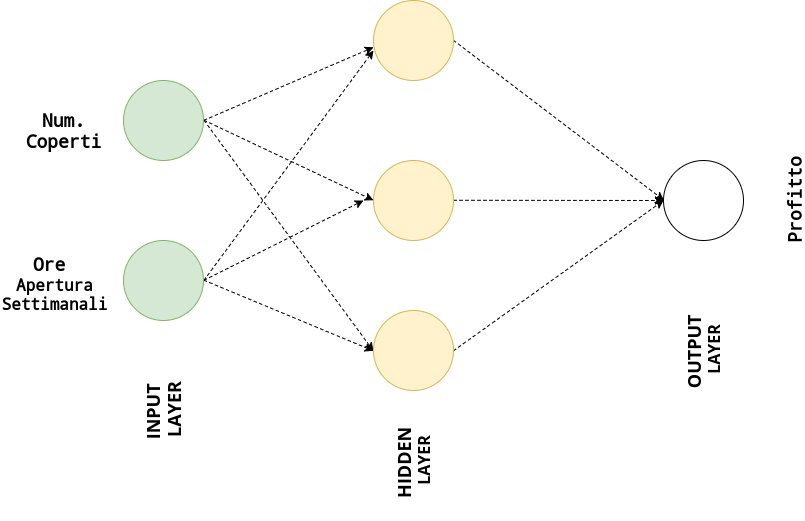
\includegraphics[width=1.0\textwidth]{\path/MLP-Profitto.png}
 \caption{Architettura del MLP per la previsione dei profitti}
 \label{fig:mlp}
\end{figure}

Di seguito gli snippet di codice per la definizione dei dati e dell'architettura della rete secondo lo schema appena presentato.

\begin{lstlisting}[language={[5.2]Lua}]
----------------------- Part 1 ----------------------------
th = require 'torch'
bestProfit = 6.0
-- X = (num coperti, ore di apertura settimanali), y = profitto lordo annuo in percentuale
torch.setdefaulttensortype('torch.DoubleTensor')
X = th.Tensor({{22,42}, {25,38}, {30,40}})
y = th.Tensor({{2.8},{3.4},{4.4}})

--normalize
normalizeTensorAlongCols(X)
y = y/bestProfit

\end{lstlisting}

\begin{lstlisting}[language={[5.2]Lua}]
----------------------- Part 2 ----------------------------
--creating the NN class in Lua, using a nice class utility
class=require 'class'
local Neural_Network = class('Neural_Network')

function Neural_Network:__init(inputs, hiddens, outputs)
      self.inputLayerSize = inputs
      self.hiddenLayerSize = hiddens
      self.outputLayerSize = outputs
      self.W1 = th.randn(net.inputLayerSize, self.hiddenLayerSize)
      self.W2 = th.randn(net.hiddenLayerSize, self.outputLayerSize)
end
\end{lstlisting}

\section{Forward Propagation}

%%% MULTI-COLUMN table for variables
\begin{table}[h!]
\caption{Variabili usate nel testo e nel codice}
\label{tab:variabili}
\begin{center}
\begin{tabular}{ |p{3cm}||p{3cm}|p{3cm}|p{3cm}|  }
 \hline
 \multicolumn{4}{|c|}{\textbf{Variabili}} \\
 \hline
 \textbf{S. Codice} & \textbf{S. Matematico} & \textbf{Definizione} & \textbf{Dimensione}\\
 \hline
 X	& $X$	&Esempi, 1 per riga&	\makecell{(numEsempi, \\inputLayerSize)}\\
 \hline
 y&	$y$	& uscita desiderata	& \makecell{(numEsempi, \\outputLayerSize)}\\
 \hline
 W1 & $W^{(1)}$	& Pesi layer 1&	\makecell{(inputLayerSize, \\hiddenLayerSize)}\\
 \hline
 W2	& $W^{(2)}$   & Pesi layer 2&	(hiddenLayerSize, outputLayerSize)\\
 \hline
 z2 & $z^{(2)}$	& Input layer 2& \makecell{(numEsempi, \\hiddenLayerSize)}\\
 \hline
 a2 & $a^{(2)}$	& Uscita layer 2& \makecell{(numEsempi, \\hiddenLayerSize)}\\
 \hline
 z3 & $z^{(3)}$	& Input layer 3& \makecell{(numEsempi, \\outputLayerSize)}\\
  \hline
 \end{tabular}
 \end{center}
 \end{table}
Nella tabella \ref{tab:variabili} sono elencate le variabili della rete. Gli input dei layer indicati con $z$ possono anche essere chiamati "attività dei layer" (indicando l'attività sulle loro sinapsi); e $a^{(2)}$ indica l'uscita del neurone dopo aver applicato la sommatoria e la funzione di attivazione sulle attività provenienti dal layer precedente.

Per muovere i dati in parallelo attraverso la rete si usa la moltiplicazione fra matrici, per questo è molto comodo usare framework che supportano operazioni fra matrici come \emph{Torch, Numpy o Matlab}. Per prima cosa, gli input del tensore $X$ devono essere moltiplicati e sommati con i pesi del primo layer $W^{(1)}$, ottenendo l'ingresso per l'hidden layer:
\begin{equation}
z^{(2)} = XW^{(1)} \tag{1}
\end{equation}
Si noti che $z^{(2)}$ è di dimensione 3x3, essendo $X$ e $W^{(1)}$ di dimensione 3x2 e 2x3 rispettivamente. \\
Ora bisogna applicare la funzione di attivazione a $z^{(2)}$. Vi sono diverse funzioni di attivazione utilizzate per le reti neurali. Una delle prime a diventare popolare fu la funzione \emph{sigmoide}\parencite{WSigmoid}, utilizzata per questa rete. Vedremo nei capitoli successivi funzioni più efficaci.
\begin{equation}
a^{(2)} = f(z^{(2)}) \tag{2},\quad ove \quad f=sigmoide
\end{equation}
Per completare la \emph{forward propagation}, bisogna seguire lo stesso procedimento per lo strato di output: sommare i contributi provenienti dall'hidden layer ed applicare la sigmoide:
\begin{center}
\begin{align*}
z^{(3)} = a^{(2)}W^{(2)} \tag{3}\\
\hat{y} = f(z^{(3)}) \tag{4}
\end{align*}
\end{center}
Essendo $a^{(2)}$ di dimensione 3x3 e $W^{(2)}$ 3x1 l'output $\hat{y}$ sarà anch'esso di dimensione 3x1, risultando quindi in una previsione per ogni esempio in ingresso. \\
Si noti come la moltiplicazione fra matrici renda tutto esprimibile in poche righe di codice.
\begin{lstlisting}[language={[5.2]Lua}]
--Note: I didn't implement manually the sigmoid function as Torch has one built-in.
--define a forward method
function Neural_Network:forward(X)
   --Propagate inputs though network
   self.z2 = th.mm(X, self.W1) --matrix multiplication
   self.a2 = th.sigmoid(self.z2)
   self.z3 = th.mm(self.a2, self.W2)
   yHat = th.sigmoid(self.z3)
   return yHat
end
\end{lstlisting}
\section{Backpropagation}
\label{sec:backprop}
Come si fa ad addestrare una rete multistrato con diversi neuroni per strato, ognuno dei quali con uscita non lineare? Tramite l'algoritmo di \emph{backpropagation of errors}, ideato da Rumelhart-Hinton-Williams nel 1985.

Non si può introdurre l'algoritmo di \emph{"backprop"} senza prima spiegare il concetto di funzione di costo (o \emph{loss function}). Nelle reti neurali (e più specificatamente nell'apprendimento supervisionato\parencite{WSupervised}, si veda anche sezione \ref{sec:training}), la funzione di costo misura la discrepanza tra l'uscita desiderata e l'effettivo output della rete. È quindi una misura dell'errore della rete, per cui l'obiettivo dell'apprendimento è trovare il minimo di questa funzione (modificando la struttura interna della rete, ovvero i pesi sinaptici).
Come per la funzione di attivazione, anche in questo caso ci sono ampie possibilità di scelta \parencite{WLoss} a seconda del task su cui la rete viene addestrata. \\
E di nuovo, come per la funzione di attivazione, si è scelta una delle funzione di costo più popolari: l'errore quadratico medio.
\begin{equation}
J = \sum_{j=1}^{n} \frac{1}{2} (y-\hat{y})^2} \tag{5}
\end{equation}
Da cui, il codice in Lua:
\begin{lstlisting}[language={[5.2]Lua}]
function Neural_Network:costFunction(X, y)
   --Compute the cost for given X,y, use weights already stored in class
   self.yHat = self:forward(X)
   J = 0.5 * th.sum(th.pow((y-yHat),2))
   return J
end
\end{lstlisting}

La \emph{backprop} ha alcuni requisiti:
\begin{itemize}
\item Reti stratificate
\item Ingressi a valori reali $\in [0,1]$
\item Neuroni non lineari con funzione di uscita sigmoidale (o altra fz. di attivazione derivabile)
\end{itemize}
Sotto queste condizioni l'algoritmo sfrutta la regola della catena\parencite{WChain} per la derivazione di funzione composte, per calcolare il gradiente della \emph{funzione di costo}. I pesi della rete vengono quindi aggiornati secondo la \emph{discesa del gradiente} (figura\ref{fig:gradDescend}); ovvero variano in maniera tale da minimizzare la funzione di costo $J$.
\begin{figure}[h!]
 \centering
 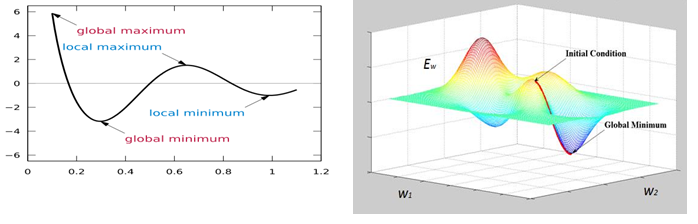
\includegraphics[width=1.0\textwidth]{\teoria/gradientbased.png}
 \caption{Cercare il minimo di una fz. seguendo la discesa del gradiente}
 \label{fig:gradDescend}
\end{figure}

Viene chiamato \emph{backward propagation of errors} poiché l'errore calcolato a partire dall'output della rete viene distribuito in maniera proporzionale all'indietro, su tutti i neuroni della rete. È importante quindi, spezzare il calcolo del gradiente dell'errore in derivate parziali, dall'ultimo strato fino al primo, e poi combinarle insieme.

Si noti che le equazioni (1-5) formano una un'unica equazione che lega $J$ a $X, y, W^{(1)}, W^{(2)}$. Tenendo questo in mente, si applica la regola della catena. \\
%% mettere la formula completa da spezzare in passaggi %%
Partendo dal fattore riguardante lo strato di output si ha:
$$
\frac{\partial J}{\partial W^{(2)}} = \sum \frac{\partial \frac{1}{2}(y-\hat{y})^2}{\partial W^{(2)}}
$$
Sviluppando i calcoli si ottiene:
$$
\frac{\partial J}{\partial W^{(2)}} = -(y-\hat{y}) \frac{\partial \hat{y}}{\partial W^{(2)}}
$$
L'equazione (4) indica che $\hat{y}$ è la funzione di attivazione di $z^{(3)}$. Da cui:
$$
\frac{\partial J}{\partial W^{(2)}} =
-(y-\hat{y})
\frac{\partial \hat{y}}{\partial z^{(3)}}
\frac{\partial z^{(3)}}{\partial W^{(2)}}
$$
Il 2° membro dell'equazione è semplicemente la derivata della funzione di attivazione sigmoide (fig. \ref{fig:sigmoidPrime}):
\begin{align*}
f(z) = \frac{1}{1+e^{-z}}\\
f^\prime(z) = \frac{e^{-z}}{(1+e^{-z})^2}
\end{align*}
Definiamola, quindi, nel codice:
%% qui codice %%
\begin{lstlisting}[language={[5.2]Lua}]
function Neural_Network:d_Sigmoid(z)
   --Derivative of sigmoid function
   return th.exp(-z):cdiv( (th.pow( (1+th.exp(-z)),2) ) )
end
\end{lstlisting}
%% qui grafico uguale al iPython %%
\begin{figure}[h!]
 \centering
 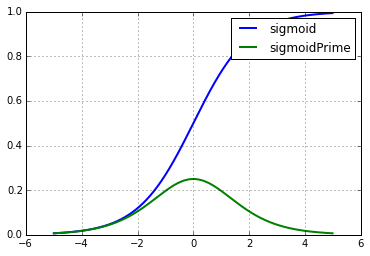
\includegraphics[width=0.5\textwidth]{\path/sigmoidPrime.png}
 \caption{La funzione sigmoide e la sua derivata}
 \label{fig:sigmoidPrime}
\end{figure}

L'equazione così ottenuta è:
$$
\frac{\partial J}{\partial W^{(2)}}=
-(y-\hat{y}) f^\prime(z^{(3)}) \frac{\partial z^{(3)}}{\partial W^{(2)}}
$$

Infine, dobbiamo trovare $\frac{\partial z^{(3)}}{\partial W^{(2)}}$, che rappresenta la variazione dell'attività del terzo layer rispetto ai pesi del secondo layer. Richiamando l'equazione (3):
$$
z^{(3)} = a^{(2)}W^{(2)} \tag{3}\\
$$
Tralasciando per un attimo la somma tra i vari neuroni, si nota una semplice relazione lineare fra i termini, con a2 che rappresenta la pendenza. Indi:
$$
\frac{\partial z^{(3)}}{\partial W^{(2)}} = a^{(2)}
$$
Indicando con $\delta^{(3)}$, l'errore sullo strato di uscita, si ha:
$$
\delta^{(3)} = -(y-\hat{y}) f^\prime(z^{(3)})
$$
Ora bisogna moltiplicare l'errore con $a^{(2)}$. Come indicato nelle ottime dispense di CS231 di Stanford\parencite{WCS231vec}: guardare alle dimensioni delle matrici può essere utile in questo caso. Infatti per fare combaciare le dimensioni, c'è solo una maniera di calcolare la derivata qui, ed è facendo la trasposta di $a^{(2)}$:
$$
\frac{\partial J}{\partial W^{(2)}} =
(a^{(2)})^T\delta^{(3)}\tag{6}
$$
Si noti che la sommatoria che abbiamo tralasciato all'inizio del calcolo viene inclusa "automaticamente" dalle somme delle moltiplicazione fra matrici.

L'ultimo termine da calcolare è $\frac{\partial J}{\partial W^{(1)}}$.
Il calcolo è inizialmente simile a quello precedente, iniziando sempre dalla derivata sull'ultimo strato ed utilizzando i risultati trovati in precedenza:
$$
\frac{\partial J}{\partial W^{(1)}} = (y-\hat{y})
\frac{\partial \hat{y}}{\partial W^{(1)}}
$$

$$
\frac{\partial J}{\partial W^{(1)}} = (y-\hat{y})
\frac{\partial \hat{y}}{\partial z^{(3)}}
\frac{\partial z^{(3)}}{\partial W^{(1)}}
$$

$$
\frac{\partial J}{\partial W^{(1)}} = -(y-\hat{y}) f^\prime(z^{(3)}) \frac{\partial z^{(3)}}{\partial W^{(1)}}
$$
$$
\frac{\partial J}{\partial W^{(1)}} = \delta^{(3)} \frac{\partial z^{(3)}}{\partial W^{(1)}}
$$
Ora rimane l'ultimo termine da calcolare, anch'esso da scomporre in diversi fattori andando a ritroso nella rete:
$$
\frac{\partial z^{(3)}}{\partial W^{(1)}} = \frac{\partial z^{(3)}}{\partial a^{(2)}}\frac{\partial a^{(2)}}{\partial W^{(1)}}
$$
Come prima, c'è una relazione lineare tra le sinapsi, ma stavolta la pendenza è data da $W_{(2)}$; anche in questo caso da trasporre.
$$
\frac{\partial J}{\partial W^{(1)}} = \delta^{(3)}
(W^{(2)})^{T}
\frac{\partial a^{(2)}}{\partial W^{(1)}}
$$
$$
\frac{\partial J}{\partial W^{(1)}} = \delta^{(3)}
(W^{(2)})^{T}
\frac{\partial a^{(2)}}{\partial z^{(2)}}
\frac{\partial z^{(2)}}{\partial W^{(1)}}
$$
$\frac{\partial a^{(2)}}{\partial z^{(2)}}$ è di nuovo la derivata della $f$ di attivazione. Il termine finale del calcolo $\frac{\partial z^{(2)}}{\partial W^{(1)}}$, rappresenta quanto varia l'uscita del primo strato al variare dei pesi. Richiamando l'equazione (1) si nota subito che questo valore è dato dal vettore di input $X$ - come prima - traposto:
$$
\frac{\partial J}{\partial W^{(1)}} =
X^{T}
\delta^{(3)}
(W^{(2)})^{T}
f^\prime(z^{(2)})
$$
Chiamando $\delta^{(2)} = \delta^{(3)} (W^{(2)})^{T} f^\prime(z^{(2)})$ diventa:
$$
\frac{\partial J}{\partial W^{(1)}} =
X^{T}\delta^{(2)} \tag{7}
$$

Facendo un sommario:

\begin{equation}
\boxed{\frac{\partial J}{\partial W^{(2)}} =
(a^{(2)})^T\delta^{(3)}\tag{6}}
\end{equation}
\begin{equation}
\boxed{\frac{\partial J}{\partial W^{(1)}} =
X^{T}\delta^{(2)} \tag{7}}
\end{equation}
\begin{equation}
\boxed{\delta^{(2)} = \delta^{(3)} (W^{(2)})^{T} f^\prime(z^{(2)}) \tag{8}}
\end{equation}
\begin{equation}
\boxed{\delta^{(3)} = -(y-\hat{y}) f^\prime(z^{(3)})  \tag{9}} \end{equation}

Implementando le equazioni sovrascritte in Lua, la classe \texttt{Neural\_Network} è quindi completa (per i dettagli si veda l'appendica \ref{AppendixA}).

\begin{lstlisting}[language={[5.2]Lua}]
function Neural_Network:d_CostFunction(X, y)
   --Compute derivative wrt to W and W2 for a given X and y
   self.yHat = self:forward(X)
   delta3 = th.cmul(-(y-self.yHat), self:d_Sigmoid(self.z3))
   dJdW2 = th.mm(self.a2:t(), delta3)

   delta2 = th.mm(delta3, self.W2:t()):cmul(self:d_Sigmoid(self.z2))
   dJdW1 = th.mm(X:t(), delta2)

   return dJdW1, dJdW2
end
\end{lstlisting}

\section{Verifica numerica del gradiente}
\label{sec:gradcheck}
Siccome la Backprop è notoriamente difficile da debuggare, una volta che la si usa per l'addestramento di una rete, bisogna controllare se l'implementazione della sezione precedente è corretta prima di proseguire nel progetto. A questo scopo, è stata scritta una funzione per il calcolo \emph{numerico} del gradiente che andrà poi confrontata con il calcolo computato dalla Backprop.

L'algoritmo\parencite{WGradcheck} è basato sulla seguente definizione di derivata:
$$
\frac{\mathrm{d} }{\mathrm{d} \theta}J(\theta)) = \lim_{\epsilon\rightarrow 0} \frac{J(\theta + \epsilon)- J(\theta - \epsilon)}{2*\epsilon}
$$
Il gradiente che bisogna controllare è formato dai 2 vettori che contengono le derivate dei pesi di tutta la rete: $\frac{\partial J}{\partial W^{(1)}} \quad e \quad \frac{\partial J}{\partial W^{(2)}}}$.\\
Approssimando $\epsilon$ con un valore molto piccolo \emph{(i.e. $10^{-4}$)} è possibile perturbare singolarmente i singoli pesi della rete (contenuti nei vettori $W_{(1)}$ e $W_{(2)}$) e calcolare così il gradiente in maniera numerica.

Per poterlo fare, servono delle funzioni ausiliare (metodi getter e setter) per prendere e settare i pesi ed il gradiente della rete come singolo vettore "flat" di parametri (appendice \ref{AppendixA}). Dopodiché basta un loop ed un array per memorizzare le derivate dei singoli pesi così calcolati:

\begin{lstlisting}[language={[5.2]Lua}]
function computeNumericalGradient(NN, X, y)
   paramsInitial = NN:getParams()
   numgrad = th.zeros(paramsInitial:size())
   perturb = th.zeros(paramsInitial:size())
   e = 1e-4

   for p=1,paramsInitial:nElement() do
      --Set perturbation vector
      perturb[p] = e
      NN:setParams(paramsInitial + perturb)
      loss2 = NN:costFunction(X, y)

      NN:setParams(paramsInitial - perturb)
      loss1 = NN:costFunction(X, y)

      --Compute Numerical Gradient
      numgrad[p] = (loss2 - loss1) / (2*e)

      --Return the value we changed to zero:
      perturb[p] = 0
   end

   --Return Params to original value:
   NN:setParams(paramsInitial)
   return numgrad
end
\end{lstlisting}
Si può ora inizializzare una rete, eseguire la backpropagation e confrontare i valori con quelli calcolati numericamente:
\begin{lstlisting}[language={[5.2]Lua}]
--test if we actually make the calculations correctly
NN = Neural_Network(2,3,1)

print('Gradient checking...')
numgrad = computeNumericalGradient(NN, X, y)
grad = NN:computeGradients(X, y)
--[[
In order to make an accurate comparison of the 2 vectors
we can calculate the difference as the ratio of:
numerator  --> the norm of the difference
denumerator--> the norm of the sum
Should be in the order of 10^-8 or less
--]]
diff = th.norm(grad-numgrad)/th.norm(grad+numgrad)
print(string.format('The difference is %e',diff))
\end{lstlisting}

Per calcolare \emph{quanto} siano effettivamente uguali i due gradienti si può usare un rapporto basato sulla norme della somma e della differenza dei gradienti (si veda il codice sopra). Se la backprop è stata implementata correttamente questa differenza dovrebbe essere nell'ordine di $10^{-8}$ o inferiore. Difatti, quando si esegue lo script si ottiene:


%%inserire figura %%
\begin{lstlisting}
$ th 4_gradCheck.lua 
Gradient checking...	
The difference is 2.123898e-10	
\end{lstlisting}

\section{Addestramento}
\label{ref:training}
%--------------------------------------------------------------------%--------------------
%	SECTION 5
%--------------------
%--------------------------------------------------------------------
Una volta accertati che l'implementazione della Backprop è corretta si può procedere ad addestrare la rete. Quello che si vuole ottenere è una rete che guardando ai dati accumulati negli anni, riesca a prevedere l'andamento del profitto del ristorante. Nel nostro dataset, ogni esempio è formato da una coppia \emph{<n. coperti, n. ore settimanali>} a cui è associata un'uscita\emph{desiderata}. La rete cercherà di modificare la sua struttura interna (i.e. i pesi sinaptici) "creando" una funzione - la rete stessa rappresenta questa funzione - per riprodurre in maniera più precisa possibile quest'associazione. L'apprendimento sarà quindi di tipo \emph{supervisionato}.
%% parlare del supervised learning e aggiungere grafico %%
\subsection{Apprendimento supervisionato}
Con questo termine s'intende l'allenamento di un sistema tramite una serie di esempi ideali; l'insieme di questi esempi è chiamato
\emph{training set}. Il sistema impara quindi ad approssimare una funzione non nota a priori a partire da una serie di coppie ingresso-uscita: per ogni input in ingresso gli si comunica l'output desiderato.
L'apprendimento consiste nella capacità del sistema – tramite la funzione generata con l'allenamento – di generalizzare a nuovi esempi: avendo in ingresso dati non noti deve poter predire in modo corretto l'output desiderato.
Matematicamente parlando, questi esempi non noti sono punti del dominio che non fanno parte dell'insieme degli esempi di training.
Esistono diversi algoritmi di apprendimento supervisionato ma tutti condividono una caratteristica: l'addestramento
viene eseguito mediante la minimizzazione di una funzione di costo (si veda la sezione \ref{sec:backprop}).
\begin{figure}[h!]
 \centering
 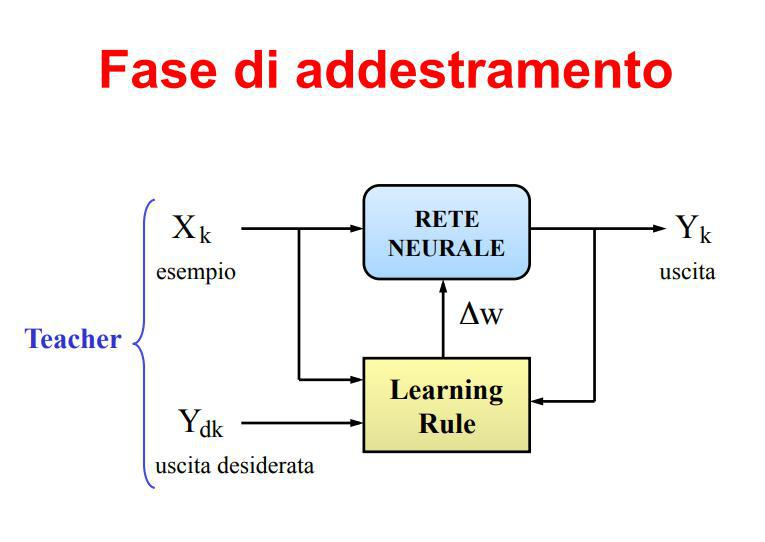
\includegraphics[width=0.8\textwidth]{\teoria/supervised-2.jpg}
 \caption{Apprendimento supervisionato: schema generale}
 \label{fig:supervised}
\end{figure}
Nella \emph{Learning Rule} in figura \ref{fig:supervised} sono compresi 2 elementi: 
\begin{enumerate}
\item Calcolo della discrepanza tra l'uscita della rete e l'uscita desiderata e backpropagation;
\item La strategia di aggiornamento dei parametri;
\end{enumerate}

Riguardo all'ultimo punto ci sono diverse possibilità. 
\subsection{Discesa del gradiente}
%% magari aggiungere un punto sul SGD%% 
La loss function è una funzione che ha un numero di variabili pari al numero dei pesi della rete. Data la complessità - soprattutto in reti profonde molto più complesse di quella trattata in questo progetto - la ricerca del minimo non è semplice; si corre il rischio di rimanere bloccati in plateau o minimi locali. Per questo, si applicano metodi a raffinamento iterativo: si parte da una soluzione iniziale e si cerca di migliorarla ad ogni ciclo. Questo metodo è conosciuto come \emph{Stochastig Gradient Descent}\parencite{WSGD}.
Calcolando il gradiente $\nabla J$ si conosce la direzione di massima variazione quindi ci si sposta - lungo l'opposto di questa direzione, l'antigradiente - di una quantità pari a $\eta$. Questo parametro si chiama \emph{learning rate} e regola appunto la velocità dell'apprendimento. 

Tornando alla strategia di aggiornamento dei parametri, la più intuitiva è chiamata \emph{"Vanilla"}: 
\begin{equation}
W_{t+1} = W_{t} - \eta \nabla J(W_t)
\end{equation}
Questa regola di apprendimento però soffre di alcuni problemi: 
\begin{itemize}
\item effettua uno spostamento pari a $\eta$ sia per features frequenti che non. Questo problema è noto come \emph{"sparsità delle features"}
\item $\eta$ è una costante e non è detto che garantisca la convergenza. Si potrebbe "saltare" da un lato all'altro del punto di minimo senza mai trovarlo. 
\item come detto sopra, i punti di sella e plateau causano problemi. In questo caso il gradiente è nullo e quindi l'aggiornamento dei pesi si azzera, fermando l'apprendimento. 
\end{itemize}

Per ovviare a questo ed altri problemi, sono stati studiati numerosi metodi. La prossima sezione ne elenca qualcuno utilizzato per questo progetto. 

\section{Ottimizzazione: diverse tecniche}
L'ottimizzazione dell'apprendimento delle reti neurali è un argomento vasto ed impervio, ma molto importante. Con addestramenti che possono durare mesi A seconda del tipo di apprendimento sono nate, in relativamente breve tempo, moltissimi metodi di ottimizzazione. Qui si faranno solo dei cenni ai metodi utlizzati in questo progetto. 

Prima di elencare tecniche più evolute dell'aggiornamento Vanilla, occorre precisare alcuni punti dello Stochastic Gradient Descent, essendo quest'ultimo il punto di partenza di ogni altro metodo. 

%SGD ASGD LBGFS ADAM
\begin{itemize}
\item \textsc{SGD}: lo \emph{Stochastic Gradient Descent} è, come lo descrive il nome stesso, una versione stocastica della discesa del gradiente. La discesa del gradiente standard non è scalabile, poiché il gradiente da calcolare tiene conto dell'errore quadratico calcolato \emph{su ogni singolo esempio del dataset}. Come detto poco fa, la loss function ha già di per sé un numero di variabili proporzionale alla complessità della rete; quando il dataset è molto largo, ed è tipico per problemi reali di machine learning, questo calcolo diventa inefficiente. L'SGD risolve questo problema approssimando l'operazione \emph{"gradiente - aggiornamento pesi"} da tutto il dataset al singolo esempio. Questo rende l'approssimazione molto inaccurata, ma molto veloce da elaborare. Nonostante le oscillazioni dovute all'inaccuratezza, questo metodo consente nella pratica, dopo molte iterazioni, di trovare il minimo globale. Questo è soprattutto vero per problemi su larga scala. 

Un compromesso tra il metodo standard e quello completamente stocastico è l'utilizzo di \emph{"mini-batch"}, cioè piccoli sottoinsiemi del dataset su cui viene eseguita l'iterazione di apprendimento. Se il dataset è abbastanza eterogeneo ed è ordinato in maniera randomica, il mini-batch approssima abbastanza bene l'intero dataset; di conseguenza, l'approssimazione sarà più verosimile al calcolo dell'intero gradiente, aumentando quindi l'accuratezza senza intaccare la velocità del calcolo. 
\item \textsc{Momentum \& NAG}: Il \emph{"Momentum"} controlla la quantità d'inerzia nella modifica dei pesi sinaptici, memorizzando nell'equazione la variazione $\Delta W$ precedente:
$$
W_{t} = W_{t-1} - \eta \nabla J(W_{t})- \underbrace{\mu\nabla 
J(W_{t-1})} 
$$ 
In questo modo si riducono le oscillazioni nella ricerca della soluzioni permettendo di usare learning rate più alti. È ispirato dal momento nella Fisica, considerando il vettore dei pesi come una particella che viaggia in uno spazio parametrico e acquisice velocità nella discesa. \\
Il \emph{Nesterov Accelerated Gradient} è una versione più raffinata del Momentum update, che elabora una correzione della traiettoria calcolando il gradiente \emph{dopo} aver fatto la somma con il gradiente accumulato precedentemente. Questo  Per aiutare a capire la differenza tra i due, si guardi la figura \ref{fig:nag}.
\begin{figure}[h!]
 \centering
 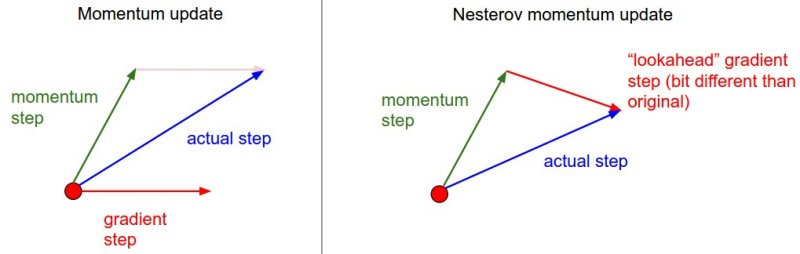
\includegraphics[width=0.8\textwidth]{\teoria/nesterov.jpg}
 \caption{Confronto tra il momentum classico e NAG}
 \label{fig:nag}
\end{figure}
\item \textsc{BFGS}: l'algoritmo \emph{Broyden-Fletcher-Goldfarb-Shanno} fa parte della famiglia "Quasi-Newton" \parencite{Wquasinewton}. Questo metodo supera i limiti della discesa del gradiente classica facendo una stima della matrice Hessiana, ovvero della curvatura della superficie della funzione di costo $J$. Utilizzando questa stima compie degli spostamenti più informati verso la discesa. Nella pratica si usa una versione efficiente che consuma meno memoria, detta Limited-BFGS\parencite{WLBFGS}. 

\item \textsc{Adam}: l'\emph{Adaptive Moment Estimation} cerca di ovviare ai problemi dell'aggiornamento vanilla modificando il learning rate in maniera diversa per ogni parametro e a seconda dello stadio dell'apprendimento. Fa parte quindi della famiglia dei metodi \emph{adattivi}. In particolare, l'algoritmo calcola la media con decadimento esponenziale del gradiente e del quadrato del gradiente; i parametri $\beta_1$ e $\beta_2$ controllano il decadimento di queste medie mobili. Gli autori forniscono i valori consigliati per questi parametri, che sono infatti i valori di default anche in ogni framework che supporta Adam\parencite{WAdam}.
\end{itemize}

Per riuscire effettivamente ad addestrare la rete, si è utilizzato un package di ottimizzazione di Torch: \texttt{optim}. Quest'ultimo fornisce il supporto a tutte (e più) le tecniche di ottimizzazione viste prima. 
Si può quindi procedere all'addestramento della rete. Utilizzando un \emph{logger} per mantenere tutti i dati sul training, si possono successivamente plottare le diverse curve di apprendimento per confrontare i diversi metodi. \\
Definita quindi una classe \texttt{Trainer}, si definisce un metodo per addestrare la rete che astrae dalla tecnica di ottimizzazione utilizzata. 
\begin{lstlisting}[language={[5.2]Lua}]
Trainer = class('Trainer')
function Trainer:__init(NN)
  --Make Local reference to network:
  self.N = NN
end

--Let's train!
function Trainer:train(X, y)
   --variables to keep track of the training
   local neval = 0
   --get initial params
   params0 = self.N:getParams()
   -- create closure to evaluate f(X) and df/dX
   -- this is requested by the API of the optim package
   local feval = function(params0)
      local f = self.N:costFunction(X, y)
      print(f)
      local df_dx = self.N:computeGradients(X, y)
      neval = neval + 1
      logger:add{neval, f} --,timer:time().real}
      return f, df_dx
   end
   if optimMethod == optim.cg then
      newparams,_,_ = optimMethod(feval, params0, optimState)
   else
      for i=1,opt.maxIter do
         newparams,_,_ = optimMethod(feval, params0, optimState)
         self.N:setParams(newparams)
      end
   end
end
\end{lstlisting}

Procedendo iterativamente con le diverse tecniche di ottimizzazione si ottiene il risultato in figura \ref{fig:comparison}. 

%INSERIRE GRAFICI
\begin{figure}[h!]
 \centering
 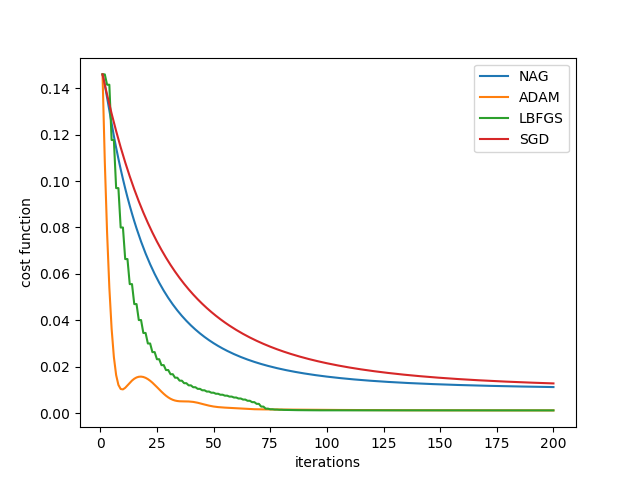
\includegraphics[width=1.0\textwidth]{\path/comparison.png}
 \caption{Confronto dei metodi di ottimizzazione durante il training}
 \label{fig:comparison}
\end{figure}
Dal grafico si evidenzia come le premesse teoriche dei vari metodi siano state pienamente rispettate. Nonostante il problema sia molto semplice se comparato ai reali problemi di \emph{deep learning}, già su un dataset ed un numero di iterazioni così limitato si nota la superiorità di un metodo verso il precedente. In particolare, nel corso \texttt{"CS231"} di deep learning applicato alla visione artificiale di Stanford\parencite{WCS231adam}, sviluppato da Andrej Karpathy et. al, si raccomanda Adam come metodo di default per applicazioni di deep learning: 
\begin{quote}
\emph{In practice Adam is currently recommended as the default algorithm to use. However, it is often also worth trying SGD+Nesterov Momentum as an alternative}.
\end{quote}

La rete è ora addestrata: dando in ingresso la matrice $X$ di input si avranno in output previsioni molto più accurate, come mostrato in figura \ref{fig:previsioni}. 
\begin{figure}[h!]
 \centering
 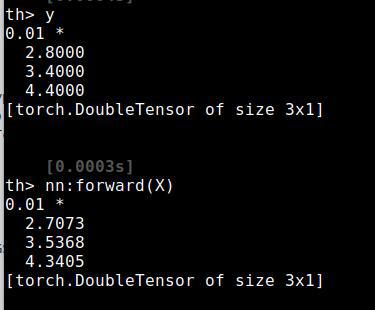
\includegraphics[width=0.5\textwidth]{\path/previsioni.jpg}
 \caption{L'output della rete $\hat{y}$ è vicino all'output desiderato $y$}
 \label{fig:previsioni}
\end{figure}

%--------------------------------------------------------------------%--------------------
%	SECTION 6
%--------------------
%--------------------------------------------------------------------
\section{Overfitting}
Uno dei problemi più comuni dell'apprendimento automatico è \emph{l'Overfitting}. Esso si verifica laddove il modello creato per fare predizioni risulta troppo complesso e troppo "legato" al solo training set, di cui apprende anche i rumori: la rete è quindi incapace di \emph{generalizzare} ad esempi ancora non visti e, nonostante l'accuratezza estremamente alta sul training set, darà delle pessime predizioni. Questo può essere dovuto a diversi fattori, di cui i più classici sono: 
\begin{itemize}
\item il modello ha troppi parametri rispetto al numero di osservazioni; 
\item il dataset è costituito da troppi pochi esempi; 
\item l'addestramento è stato fatto troppo a lungo;
\end{itemize}

In figura \ref{fig:regularization} è mostrato un esempio di 2 modelli statistici che hanno entrambi errore nullo ma complessità molto diversa. 
\begin{figure}[h!]
 \centering
 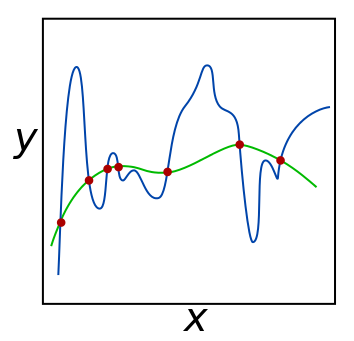
\includegraphics[width=0.6\textwidth]{\path/reg-wikipedia.png}
 \caption{Entrambe le funzioni hanno un'errore nullo sul dataset. Tuttavia, la funzione blu è eccessivamente complessa ed affetta da rumore; avrà quindi cattive capacità di generalizzazione. La verde, al contrario, sarà presumibilmente più corretta rispetto ai punti sconosciuti della distribuzione sottostante.}
 \label{fig:regularization}
\end{figure}
\subsection{Rilevare l'overfitting}
Per rilevare se è avvenuto o meno overfitting durante l'apprendimento; si possono dare in ingresso al percettrone esempi ancora non visti e controllare "ad occhio" se le predizioni hanno senso. Per averne la certezza però, bisogna dividere il dataset in un training set ed un \emph{test set} su cui testare la rete durante l'apprendimento. Sugli esempi del test set non si farà backpropagation e non avverrà quindi apprendimento; si utilizzeranno solo per sapere quanto è corretto l'addestramento. \\
Testando la rete \emph{durante} l'apprendimento si può capire il preciso momento in cui avviene l'overfitting. Per farlo, occorre plottare sullo stesso grafico l'errore sul training set e sul test set. 

Dopo aver definito arbitrariamente alcuni esempi di testing, si modifica l'algoritmo di training: 
\begin{lstlisting}[language={[5.2]Lua}]
--Need to modify trainer class a bit to check testing error during training:
function Trainer:train(trainX, trainY, testX, testY)
   --variables to keep track of the training
   local neval = 0

   params0 = self.N:getParams()
   -- create closure to evaluate f(X) and df/dX
   local feval = function(params0)
      local f = self.N:costFunction(trainX, trainY)
      local test = self.N:costFunction(testX, testY)
      --printing training and testing error
      print(f..' '..test)
      local df_dx = self.N:computeGradients(trainX, trainY)
      neval = neval + 1
      --logging both training and testing data
      logger:add{neval, f} --,timer:time().real}
      testLogger:add{neval, test}

      return f, df_dx
   end

   if optimMethod == optim.cg then
      newparams,_,_ = optimMethod(feval, params0, optimState)
   else
      for i=1,opt.maxIter do
         newparams,_,_ = optimMethod(feval, params0, optimState)
         self.N:setParams(newparams)
      end
   end
end
\end{lstlisting}

Si addestra la rete e si loggano i valori di training e di testing: 
\begin{lstlisting}[language={[5.2]Lua}]
--now let's train and check where exactly the net is Overfitting
nn = Neural_Network(2,3,1)

init_params = nn:getParams()
logtrain = 'train.log'
logtest = 'test.log'
logger = optim.Logger(logtrain)
testLogger = optim.Logger(logtest)

trainer = Trainer(nn)
trainer:train(trainX, trainY, testX, testY)
\end{lstlisting}

Andando infine a plottare i dati così ottenuti, si osserva la presenza di overfitting: 
\begin{figure}[h!]
 \centering
 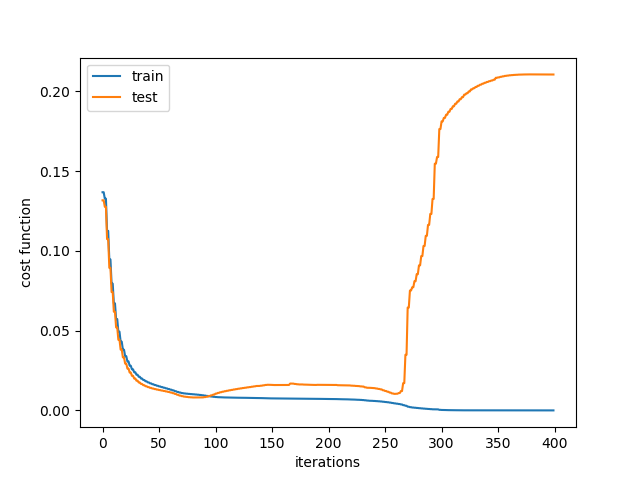
\includegraphics[width=0.6\textwidth]{\path/overfitting.png}
 \caption{La rete mostra overfitting. Dopo l'iterazione 100 le performance sul test set iniziano ad essere sbagliate. Attorno alla 250 il modello diventa troppo complesso e le predizioni sono pessime}
 \label{fig:overfitting}
\end{figure}


\subsection{Contromisure}
Vi sono diverse contromisure contro l'overfitting, che seguono le cause più comuni: 
\begin{itemize}
\item dataset più ampio: una regola empirica consiste nell'avere circa 10 esempi per ogni parametro della rete. Nel caso del MLP di questo progetto i pesi sono 9, quindi secondo questa regola sono necessari 90 esempi. È ovvimente impossibile, poiché Loris ha collezionato solamente un limitato numero di esempi. 
\item \emph{k-fold cross-validation}: si divide il dataset in K set di eguale misura, ad ogni iterazione uno dei set viene utilizzato come test-set ed il resto viene per formare il training e validation set (si veda lez.1 del corso di Machine Learning per PhD di M. Lippi\prencite{WLippi}). Anche questa procedura non è applicabile in questo caso. 
\item \emph{Dropout}: il dropout è una tecnica di regolarizzazione maggiormente utilizzata nelle reti profonde, nella quale ad ogni iterazione si "spengono" alcuni neuroni (settando i pesi che li collegano a 0). Questo fa sì che neuroni vicini non si specializzino tutti a riconoscere le stesse caratteristiche, risultando in un minore overfitting. Una spiegazione approfondita esula dallo scopo di questo elaborato, per cui si suggerisce la consultazione del paper di Srivastava, Hinton et. al\parencite{Dropout}.  
\item arresto anticipato: una volta rilevato quando avviene precisamente l'overfitting, si arresta l'apprendimento \emph{prima} di quel momento. Osservando la figura \ref{fig:overfitting} si potrebbe pensare di fermare le iterazioni alla n.100 (o comunque prima della n. 250) e funzionerebbe. Così facendo, si ha una maniera piuttosto semplice di risolvere il problema. C'è uno svantaggio però: se la rete non è ancora ben addestrata non c'è possibilità di migliorarla ulteriormente, poiché ogni nuova iterazione causerebbe overfitting. Per questo, è stato usato l'ultimo metodo qui presentato. 
\item Regolarizzazione: consiste nell'aggiungere un termine alla funzione di costo $J$ che penalizza modelli troppo complessi. \parencite{WLippi}. Questo termine, $\lambda R(W)$ è regolato da un parametro $\lambda$ che definisce l'intensità della regolarizzazione. 
\end{itemize}\\
Un comune metodo di regolarizzazione è la \emph{L2 Regularization}: si implementa aggiungendo alla funzione di costo il quadrato dei tensori dei pesi della rete. In questa maniera si tengono i valori di tutti i pesi piuttosto bassi evitando che si specializzino troppo sui dati del training set. Di seguito il codice dei metodi della rete che devono essere modificati:  
\begin{lstlisting}[language={[5.2]Lua}]
--[[
## Introducing a Regularization term to mitigate overfitting ## 
Lambda will allow us to tune the relative cost: 
higher values of Lambda --> bigger penalties for high model complexity 
--]]

--so, the new Neural_Network class now becomes:
Neural_Network = class(function(net, inputs, hiddens, outputs, lambda)
      net.inputLayerSize = inputs
      net.hiddenLayerSize = hiddens
      net.outputLayerSize = outputs
      net.W1 = th.randn(net.inputLayerSize, net.hiddenLayerSize)
      net.W2 = th.randn(net.hiddenLayerSize, net.outputLayerSize)

      --regularization parameter
      net.lambda = lambda
   end)

function Neural_Network:costFunction(X, y)
   --Compute the cost for given X,y, use weights already stored in class
   self.yHat = self:forward(X)
   J = 0.5 * th.sum(th.pow((y-yHat),2))/X:size()[1] + 
            (self.lambda/2) * (th.sum(th.pow(self.W1,2)) + th.sum(th.pow(self.W2, 2)))

   return J
end

function Neural_Network:d_costFunction(X, y)
   --Compute derivative wrt to W and W2 for a given X and y
   self.yHat = self:forward(X)
   delta3 = th.cmul(-(y-self.yHat), self:d_Sigmoid(self.z3))
   --Add gradient of regularization term:
   dJdW2 = th.mm(self.a2:t(), delta3)/X:size()[1] + self.lambda*self.W2

   delta2 = th.mm(delta3, self.W2:t()):cmul(self:d_Sigmoid(self.z2))
   --Add gradient of regularization term:
   dJdW1 = th.mm(X:t(), delta2)/X:size()[1] + self.lambda*self.W1

   return dJdW1, dJdW2
end
\end{lstlisting}
\linebreak
Eseguendo ora l'addestramento si ottengono risultati in figura \ref{fig:reg-plot}. Si può osservare come la regolarizzazione sia stata efficace e le 2 curve siano pressoché identiche. Si noti anche che, data la modesta complessità del problema, dopo circa la 130esima iterazione si è già raggiunto un minimo ed il processo di apprendimento non migliora ulteriormente. 
\begin{figure}[h!]
 \centering
 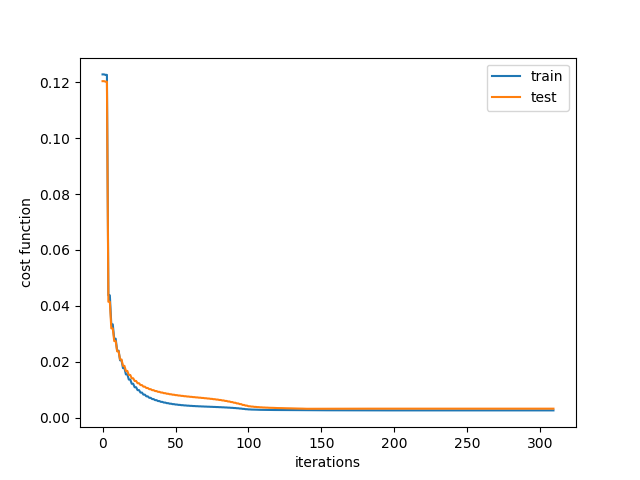
\includegraphics[width=0.65\textwidth]{\path/regularization.png}
 \caption{Dopo aver applicato la L2 regularization, la rete non è più affetta da overfitting.}
 \label{fig:reg-plot}
\end{figure}

%%inserire grafico ultimo

%--------------------------------------------------------------------%--------------------
%	SECTION 7
%--------------------
%--------------------------------------------------------------------
\newpage
\section{Risultati}
In questo capitolo si è visto come costruire da zero l'architettura di un percettrone multi-strato con paradigma OOP; come implementare la backpropagation e controllare numericamente che funzioni in maniera corretta. Successivamente si sono visti i principali algoritmi per ottimizzare l'apprendimento supervisionato di una rete neurale. Si è poi affrontato il problema dell'overfitting: come rilevarlo in maniera precisa ed un introduzione alle tecniche più comuni per risolverlo. \\
Infine, si è ottenuto una rete neurale capace di predire in maniera corretta il profitto di un ristorante in base al numero di coperti ed il numero di ore di apertura settimanali. 